\documentclass[12pt]{beamer}
\usepackage[utf8]{inputenc}
\usetheme{default}
\usepackage{pgf,pgfarrows,pgfnodes}
\usepackage{graphicx}
\usepackage{algorithmicx} 
\usepackage{color}
\usepackage{lipsum}  
\usepackage{xcolor}
\usepackage{hyperref}
\usepackage[english]{babel}
\usepackage{graphicx}
\usepackage{ragged2e}
\usepackage{tikz}
\usepackage{multirow}
\usepackage{tabularx}
\usepackage{array}
\usepackage{mathptmx}       % selects Times Roman as basic font
\usepackage{helvet}         % selects Helvetica as sans-serif font
\usepackage{courier}        % selects Courier as typewriter font
\usepackage{type1cm}        % activate if the above 3 fonts are
\usepackage{textpos} 
\usepackage{pgf,pgfarrows,pgfnodes}
\usepackage{graphicx}
\usepackage{color}
\usepackage{natbib}
\setbeamersize{text margin left=10pt,text margin right=10pt}
\definecolor{idrbt_dark_blue}{HTML}{3333b3}
\definecolor{idrbt_blue}{HTML}{00AEEF} 
\definecolor{adroit_black}{HTML}{222222}
\let\oldcite=\cite                                                              
\renewcommand{\cite}[1]{\textcolor[rgb]{0,.7,0}{\oldcite{#1}}}
\setbeamercolor{item}{fg=idrbt_blue}
\setbeamertemplate{section in toc}
{\leavevmode\leftskip=2ex%
	\llap{%
		\usebeamerfont*{section number projected}%
		\usebeamercolor{section number projected}%
		\begin{pgfpicture}{-1ex}{0ex}{1ex}{2ex}
			\color{idrbt_blue}
			%      \color{red}
			\pgfpathcircle{\pgfpoint{0pt}{.75ex}}{1.7ex}
			\pgfusepath{fill}
			\pgftext[base]{\color{fg}\inserttocsectionnumber}
		\end{pgfpicture}\kern1.25ex%
	}%
	\inserttocsection\par}
\date{}
\title{\textcolor{idrbt_blue}{\rule{112mm}{1.25mm}} \textbf{Lecture-2:\\ Tables, Figures, Math \& Bibliography}
	 \textcolor{idrbt_blue}{\rule{112mm}{1.25mm}}}
\author{\textcolor{red}{\texttt{\textbf{Manu.V.T.}\\ 
			{\scriptsize Senior Research Fellow\\ Center of Excellence in Cyber Security\\IDRBT}}} }%\newline {\scriptsize Research Fellow} }
%%%%%%%%%%%%%%%%%%%%%%%%%%%%%%%%%%%%%%%%%%%%%%%%%%%%%%%%%%%%%%
\makeatletter
\long\def\beamer@section[#1]#2{%
	\beamer@savemode%
	\mode<all>%
	\ifbeamer@inlecture
	\refstepcounter{section}%
	\beamer@ifempty{#2}%
	{\long\def\secname{#1}\long\def\lastsection{#1}}%
	{\global\advance\beamer@tocsectionnumber by 1\relax%
		\long\def\secname{#2}%
		\long\def\lastsection{#1}%
		\addtocontents{toc}{\protect\beamer@sectionintoc{\the\c@section}{#2\hfill\the\c@page}{\the\c@page}{\the\c@part}%
			{\the\beamer@tocsectionnumber}}}%
	{\let\\=\relax\xdef\sectionlink{{Navigation\the\c@page}{\noexpand\secname}}}%
	\beamer@tempcount=\c@page\advance\beamer@tempcount by -1%
	\beamer@ifempty{#1}{}{%
		\addtocontents{nav}{\protect\headcommand{\protect\sectionentry{\the\c@section}{#1}{\the\c@page}{\secname}{\the\c@part}}}%
		\addtocontents{nav}{\protect\headcommand{\protect\beamer@sectionpages{\the\beamer@sectionstartpage}{\the\beamer@tempcount}}}%
		\addtocontents{nav}{\protect\headcommand{\protect\beamer@subsectionpages{\the\beamer@subsectionstartpage}{\the\beamer@tempcount}}}%
	}%
	\beamer@sectionstartpage=\c@page%
	\beamer@subsectionstartpage=\c@page%
	\def\insertsection{\expandafter\hyperlink\sectionlink}%
	\def\insertsubsection{}%
	\def\insertsubsubsection{}%
	\def\insertsectionhead{\hyperlink{Navigation\the\c@page}{#1}}%
	\def\insertsubsectionhead{}%
	\def\insertsubsubsectionhead{}%
	\def\lastsubsection{}%
	\Hy@writebookmark{\the\c@section}{\secname}{Outline\the\c@part.\the\c@section}{2}{toc}%
	\hyper@anchorstart{Outline\the\c@part.\the\c@section}\hyper@anchorend%
	\beamer@ifempty{#2}{\beamer@atbeginsections}{\beamer@atbeginsection}%
	\fi%
	\beamer@resumemode}%

\def\beamer@subsection[#1]#2{%
	\beamer@savemode%
	\mode<all>%
	\ifbeamer@inlecture%
	\refstepcounter{subsection}%
	\beamer@ifempty{#2}{\long\def\subsecname{#1}\long\def\lastsubsection{#1}}
	{%
		\long\def\subsecname{#2}%
		\long\def\lastsubsection{#1}%
		\addtocontents{toc}{\protect\beamer@subsectionintoc{\the\c@section}{\the\c@subsection}{#2\hfill\the\c@page}{\the\c@page}{\the\c@part}{\the\beamer@tocsectionnumber}}%
	}%
	\beamer@tempcount=\c@page\advance\beamer@tempcount by -1%
	\addtocontents{nav}{%
		\protect\headcommand{\protect\beamer@subsectionentry{\the\c@part}{\the\c@section}{\the\c@subsection}{\the\c@page}{\lastsubsection}}%
		\protect\headcommand{\protect\beamer@subsectionpages{\the\beamer@subsectionstartpage}{\the\beamer@tempcount}}%
	}%
	\beamer@subsectionstartpage=\c@page%
	\edef\subsectionlink{{Navigation\the\c@page}{\noexpand\subsecname}}%
	\def\insertsubsection{\expandafter\hyperlink\subsectionlink}%
	\def\insertsubsubsection{}%
	\def\insertsubsectionhead{\hyperlink{Navigation\the\c@page}{#1}}%
	\def\insertsubsubsectionhead{}%
	\Hy@writebookmark{\the\c@subsection}{#2}{Outline\the\c@part.\the\c@section.\the\c@subsection.\the\c@page}{3}{toc}%
	\hyper@anchorstart{Outline\the\c@part.\the\c@section.\the\c@subsection.\the\c@page}\hyper@anchorend%
	\beamer@ifempty{#2}{\beamer@atbeginsubsections}{\beamer@atbeginsubsection}%
	\fi%
	\beamer@resumemode}

\makeatother
%%%%%%%%%%%%%%%%%%%%%%%%%%%%%%%%%%%%%%%%%%%%%%%%%%%%%%%%%%%%%%
\beamertemplatenavigationsymbolsempty

\addtobeamertemplate{navigation symbols}{}{%
	\usebeamerfont{footline}%
	\usebeamercolor[fg]{footline}%
	\hspace{1em}%
	\insertframenumber/\inserttotalframenumber
}
%%%%%%%%%%%%%%%%%%%%%%%%%%%%%%%%%%%%%%%%%%%%%%%%%%%%%%%%%%%%%%
\begin{document}
	%%%%%%%%%%%%%%%%%%%%%%%%%%%%%%%%%%%%%%%%%%%%%%%%%%%%%%%%%%%%%%%%%%%%%%%%%%%%%%%%%%%%%%%%%%%%%%%%%%%%%%%%%%%%%%%%%%%%%%%%%%%%%
	
	\begin{frame}
	\titlepage
	


\begin{center}
			\begin{tabular}{l>{\centering}p{6.25cm}<{\centering}l}
			\multirow{1}{*}{
\includegraphics[scale=0.15]{./IDRBT_lowres.png}}
			&
         
			&
			\multirow{1}{*}{
\includegraphics[scale=0.2]{./uoh.png}}
		\end{tabular}
\end{center}

\smallskip
	\renewcommand*{\arraystretch}{1.05}



\end{frame}
%%%%%%%%%%%%%%%%%%%%%%%%%%%%%%%%%%%%%%%%%%%%%%%%%%%%%%%%%%%%%%%%%%%%%%%%%%%%%%%%%%%%%%%%%%%%%%%%%%%%%%%%%%%%%%%%%%%%%%%%%%%%%

\begin{frame}
\frametitle{Outline}
\tableofcontents %[hideallsubsections]
\end{frame}
%%%%%%%%%%%%%%%%%%%%%%%%%%%%%%%%%%%%%%%%%%%%%%%%%%%%%%%%%%%%%%%%%%%%%%%%%%%%%%%%%%%%%%%%%%%%%%%%%%%%%%%%%%%%%%%%%%%%%%%%%%%%%

%%%%%%%%%%%%%%%%%%%%%%%%%%%%%%%%%%%%%%%%%%%%%%%%%%%%%%%%%%%%%%%%%%%%%%%%%%%%%%%%%%%%%%%%%%%%%%%%%%%%%%%%%%%%%%%%%%%%%%%%%%%%%
\begin{frame}
\section{\LaTeX{} Floats}
\frametitle{\LaTeX{} Floats}
	\begin{itemize}\justifying
		\item Floats are containers for things in a document that cannot be broken over a page.
		\item \LaTeX{} by default recognizes ``table" and ``figure" floats.
		\item Positioned in a part of the page to themselves (top, middle, bottom, left, right, or wherever the designer specifies). 
		\item They always have a caption describing them and they are always numbered so they can be referred to from elsewhere in the text. 
		\item LaTeX automatically floats Tables and Figures, depending on how much space is left on the page at the point that they are processed. If there is not enough room on the current page, the float is moved to the top of the next page. 
	\end{itemize}
\end{frame}
%%%%%%%%%%%%%%%%%%%%%%%%%%%%%%%%%%%%%%%%%%%%%%%%%%%%%%%%%%%%%%%%%%%%%%%%%%%%%%%%%%%%%%%%%%%%%%%%%%%%%%%%%%%%%%%%%%%%%%%%%%%%%
%%%%%%%%%%%%%%%%%%%%%%%%%%%%%%%%%%%%%%%%%%%%%%%%%%%%%%%%%%%%%%%%%%%%%%%%%%%%%%%%%%%%%%%%%%%%%%%%%%%%%%%%%%%%%%%%%%%%%%%%%%%%%
\begin{frame}[fragile]
\section{ Tables        }
\frametitle{Tables}
			\begin{verbatim}
	\begin{table}[placement specifier]
	\label{table:1}
	\caption{}
		....contents of the table here
		\end{table}
	\end{verbatim} 
\begin{center}
	\textbf{placement specifiers}
\end{center}
\renewcommand{\arraystretch}{1.05}
\begin{tabular}{lp{0.9\textwidth}}
	\hline
	h 	&Place the float here, i.e., approximately at the same point it occurs in the source text \\\hline
	t 	&Position at the top of the page.\\\hline
	b 	&Position at the bottom of the page.\\\hline
	p 	&Put on a special page for floats only.\\\hline
	! 	&Override internal parameters LaTeX uses for determining ``good" float positions.\\\hline
	H 	&Places the float at precisely the location in the LaTeX code. This is somewhat equivalent to !ht.\\\hline
\end{tabular}
\end{frame}
%%%%%%%%%%%%%%%%%%%%%%%%%%%%%%%%%%%%%%%%%%%%%%%%%%%%%%%%%%%%%%%%%%%%%%%%%%%%%%%%%%%%%%%%%%%%%%%%%%%%%%%%%%%%%%%%%%%%%%%%%%%%%
%%%%%%%%%%%%%%%%%%%%%%%%%%%%%%%%%%%%%%%%%%%%%%%%%%%%%%%%%%%%%%%%%%%%%%%%%%%%%%%%%%%%%%%%%%%%%%%%%%%%%%%%%%%%%%%%%%%%%%%%%%%%%
\begin{frame}[fragile]
\section{    How to Create Tables?     }
\frametitle{How to Create Tables?}
\begin{itemize}
	\item Input:
	\begin{verbatim}
	\begin{tabular}{cc}
	1 &NDP\\
	2 &Prasad\\
	3 &Yashwanth\\
	4 &Raghu\\
	\end{tabular}
	\end{verbatim}
	\item Output:\\
		\begin{tabular}{cc}
			1 &NDP\\
		2 &Prasad\\
		3 &Yashwanth\\
		4 &Raghu\\
	\end{tabular}
\end{itemize}

\end{frame}
%%%%%%%%%%%%%%%%%%%%%%%%%%%%%%%%%%%%%%%%%%%%%%%%%%%%%%%%%%%%%%%%%%%%%%%%%%%%%%%%%%%%%%%%%%%%%%%%%%%%%%%%%%%%%%%%%%%%%%%%%%%%%
%%%%%%%%%%%%%%%%%%%%%%%%%%%%%%%%%%%%%%%%%%%%%%%%%%%%%%%%%%%%%%%%%%%%%%%%%%%%%%%%%%%%%%%%%%%%%%%%%%%%%%%%%%%%%%%%%%%%%%%%%%%%%
\begin{frame}
\section{         }
\frametitle{Does it Really Look Like Tables?}
Output:
\begin{center}
	\begin{tabular}{|c|c|}
		\hline
				1 &NDP\\		\hline
			2 &Prasad\\		\hline
			3 &Yashwanth\\		\hline
			4 &Raghu\\
			\hline
\end{tabular}
\end{center}
\end{frame}
%%%%%%%%%%%%%%%%%%%%%%%%%%%%%%%%%%%%%%%%%%%%%%%%%%%%%%%%%%%%%%%%%%%%%%%%%%%%%%%%%%%%%%%%%%%%%%%%%%%%%%%%%%%%%%%%%%%%%%%%%%%%%
%%%%%%%%%%%%%%%%%%%%%%%%%%%%%%%%%%%%%%%%%%%%%%%%%%%%%%%%%%%%%%%%%%%%%%%%%%%%%%%%%%%%%%%%%%%%%%%%%%%%%%%%%%%%%%%%%%%%%%%%%%%%%
\begin{frame}[fragile]
\section{         }
\frametitle{}
Input:
\begin{center}
	\begin{verbatim}
	\begin{tabular}{|c|l|}
\hline
1 &NDP\\		\hline
2 &Prasad\\		\hline
3 &Yashwanth\\		\hline
4 &Raghu\\
\hline
\end{tabular}
\end{verbatim}
\end{center}
\end{frame}
%%%%%%%%%%%%%%%%%%%%%%%%%%%%%%%%%%%%%%%%%%%%%%%%%%%%%%%%%%%%%%%%%%%%%%%%%%%%%%%%%%%%%%%%%%%%%%%%%%%%%%%%%%%%%%%%%%%%%%%%%%%%%
%%%%%%%%%%%%%%%%%%%%%%%%%%%%%%%%%%%%%%%%%%%%%%%%%%%%%%%%%%%%%%%%%%%%%%%%%%%%%%%%%%%%%%%%%%%%%%%%%%%%%%%%%%%%%%%%%%%%%%%%%%%%%
\begin{frame}
\section{Customizing Tables         }
\frametitle{Customizing Tables}
Output:
\begin{center}
	\begin{tabular}{|p{2cm}|p{4cm}|}
	\hline
	1 &NDP\\		\hline
	2 &Prasad\\		\hline
	3 &Yashwanth\\		\hline
	4 &Raghu\\
	\hline
\end{tabular}
\end{center}
\end{frame}
%%%%%%%%%%%%%%%%%%%%%%%%%%%%%%%%%%%%%%%%%%%%%%%%%%%%%%%%%%%%%%%%%%%%%%%%%%%%%%%%%%%%%%%%%%%%%%%%%%%%%%%%%%%%%%%%%%%%%%%%%%%%%
%%%%%%%%%%%%%%%%%%%%%%%%%%%%%%%%%%%%%%%%%%%%%%%%%%%%%%%%%%%%%%%%%%%%%%%%%%%%%%%%%%%%%%%%%%%%%%%%%%%%%%%%%%%%%%%%%%%%%%%%%%%%%
\begin{frame}[fragile]
\section{         }
\frametitle{Customizing Tables  }

\begin{verbatim}
	\begin{tabular}{|p{2cm}|p{4cm}|}
	\hline
1 &NDP\\		
\hline
2 &Prasad\\		
\hline
3 &Yashwanth\\		
\hline
4 &Raghu\\
\hline
\end{tabular}
\end{verbatim}

\end{frame}
%%%%%%%%%%%%%%%%%%%%%%%%%%%%%%%%%%%%%%%%%%%%%%%%%%%%%%%%%%%%%%%%%%%%%%%%%%%%%%%%%%%%%%%%%%%%%%%%%%%%%%%%%%%%%%%%%%%%%%%%%%%%%
\begin{frame}[fragile]
\section{         }
\frametitle{Customizing Tables  }
Input:
\begin{verbatim}
\begin{tabular}{l>{\centering}p{4cm}<{\centering}}
\hline
1 &NDP \tabularnewline		
\hline
2 &Prasad \tabularnewline	
\hline
3 &Yashwanth \tabularnewline	
\hline
4 &Raghu \tabularnewline
\hline
\end{tabular}
\end{verbatim}

\end{frame}
\begin{frame}[fragile]
\section{         }
\frametitle{Customizing Tables  }
Output:\\
\begin{tabular}{|r|>{\centering}p{4cm}<{\centering}|}
	\hline
1 &NDP \tabularnewline	
	\hline
2 &Prasad\tabularnewline
	\hline		
3 &Yashwanth\tabularnewline
	\hline	
4 &Raghu\tabularnewline
	\hline
\end{tabular}
\end{frame}
%%%%%%%%%%%%%%%%%%%%%%%%%%%%%%%%%%%%%%%%%%%%%%%%%%%%%%%%%%%%%%%%%%%%%%%%%%%%%%%%%%%%%%%%%%%%%%%%%%%%%%%%%%%%%%%%%%%%%%%%%%%%%
\begin{frame}[fragile]
\section{         }
\frametitle{Customizing Tables  }
Output:\\
\begin{tabular}{|r|>{\centering}p{4cm}<{\centering}|}
	\hline
	\multicolumn{2}{|c|}{My Students} \\
	\hline
	1 &NDP \tabularnewline	
	\hline
	2 &Prasad\tabularnewline
	\hline		
	3 &Yashwanth\tabularnewline
	\hline	
	4 &Raghu\tabularnewline
	\hline
\end{tabular}
\end{frame}

\begin{frame}[fragile]
\section{         }
\frametitle{Customizing Tables  }
Output:\\
\begin{verbatim}
\begin{tabular}{|r|>{\centering}p{4cm}<{\centering}|}
	\hline
	\multicolumn{2}{|c|}{My Students} \\
	\hline
	1 &NDP \tabularnewline	
	\hline
	2 &Prasad\tabularnewline
	\hline		
	3 &Yashwanth\tabularnewline
	\hline	
	4 &Raghu\tabularnewline
	\hline
\end{tabular}
\end{verbatim}
\end{frame}

\begin{frame}
\begin{tabular}{|l|r|>{\centering}p{4cm}<{\centering}|}
	\hline
	\multicolumn{3}{|c|}{My Students} \tabularnewline
	\hline
	\multirow{3}{*}{Telangana} 	& 1 & Raghu \tabularnewline
								& 2 & Prasad \tabularnewline
								& 3 & Sreedevi \tabularnewline
								\hline
	\multirow{2}{*}{UP} 		& 1 & Narotham \tabularnewline
								& 2 & Malvika Singh \tabularnewline 
								\hline
	\multirow{2}{*}{Andhra} 	& 1 & Anand \tabularnewline
								& 2 & Yaswanth \tabularnewline
								\hline
\end{tabular}
\end{frame}

\begin{frame}[shrink=20,fragile]
\section{         }
\frametitle{Customizing Tables  }

\begin{verbatim}
\begin{tabular}{|l|r|>{\centering}p{4cm}<{\centering}|}
\hline
\multicolumn{3}{|c|}{My Students} \tabularnewline
\hline
\multirow{3}{*}{Telangana} 	& 1 & Raghu \tabularnewline
							& 2 & Prasad \tabularnewline
							& 3 & Sreedevi \tabularnewline
\hline
\multirow{2}{*}{UP} 		& 1 & Narotham \tabularnewline
& 2 & Malvika Singh \tabularnewline 
\hline
\multirow{2}{*}{Andhra} 	& 1 & Anand \tabularnewline
& 2 & Yaswanth \tabularnewline
\hline
\end{tabular}
\end{verbatim}
\end{frame}
%%%%%%%%%%%%%%%%%%%%%%%%%%%%%%%%%%%%%%%%%%%%%%%%%%%%%%%%%%%%%%%%%%%%%%%%%%%%%%%%%%%%%%%%%%%%%%%%%%%%%%%%%%%%%%%%%%%%%%%%%%%%%
\begin{frame}
\section{         }
\frametitle{Table inside Table Environment}
\begin{table}
	  \centering
	\label{table:1}
		\begin{tabular}{|p{2cm}|p{4cm}|}
		\hline
		1 &NDP\\		
		\hline
		2 &Prasad\\		
		\hline
		3 &Yashwanth\\		
		\hline
		4 &Raghu\\
		\hline
	\end{tabular}
		\caption{List of PhD students attending \LaTeX{} Class}
\end{table}
\end{frame}
%%%%%%%%%%%%%%%%%%%%%%%%%%%%%%%%%%%%%%%%%%%%%%%%%%%%%%%%%%%%%%%%%%%%%%%%%%%%%%%%%%%%%%%%%%%%%%%%%%%%%%%%%%%%%%%%%%%%%%%%%%%%%
%%%%%%%%%%%%%%%%%%%%%%%%%%%%%%%%%%%%%%%%%%%%%%%%%%%%%%%%%%%%%%%%%%%%%%%%%%%%%%%%%%%%%%%%%%%%%%%%%%%%%%%%%%%%%%%%%%%%%%%%%%%%%
\begin{frame}[fragile]
\section{Figures}
\frametitle{Figures}
\begin{verbatim}
\begin{figure}[h]
\centering

\includegraphics[scale=0.5]{lion}
\caption{The \LaTeX{} Mascot}
\label{fig:lion}
\end{figure}
\end{verbatim}
\end{frame}
%%%%%%%%%%%%%%%%%%%%%%%%%%%%%%%%%%%%%%%%%%%%%%%%%%%%%%%%%%%%%%%%%%%%%%%%%%%%%%%%%%%%%%%%%%%%%%%%%%%%%%%%%%%%%%%%%%%%%%%%%%%%%\\
%%%%%%%%%%%%%%%%%%%%%%%%%%%%%%%%%%%%%%%%%%%%%%%%%%%%%%%%%%%%%%%%%%%%%%%%%%%%%%%%%%%%%%%%%%%%%%%%%%%%%%%%%%%%%%%%%%%%%%%%%%%%%
\begin{frame}
\begin{figure}[h]
	\centering
    
\includegraphics[scale=0.5]{lion}
	\caption{The \LaTeX{} Mascot}
	\label{fig:lion}
\end{figure}
\end{frame}
%%%%%%%%%%%%%%%%%%%%%%%%%%%%%%%%%%%%%%%%%%%%%%%%%%%%%%%%%%%%%%%%%%%%%%%%%%%%%%%%%%%%%%%%%%%%%%%%%%%%%%%%%%%%%%%%%%%%%%%%%%%%%
%%%%%%%%%%%%%%%%%%%%%%%%%%%%%%%%%%%%%%%%%%%%%%%%%%%%%%%%%%%%%%%%%%%%%%%%%%%%%%%%%%%%%%%%%%%%%%%%%%%%%%%%%%%%%%%%%%%%%%%%%%%%%
\begin{frame}[fragile]
\section{Formulae \& Math         }
\frametitle{Formulae \& Math }
\begin{itemize}\justifying
	\item Math mode 
	\begin{enumerate}
		\item Inline mode
		\begin{itemize}
			\item \verb|\( \), $ $ or \begin{math} \end{math}|
			\renewcommand{\arraystretch}{2}
			\begin{tabular}{|c|c|}
				\hline
				\textbf{Output} &\textbf{Input}\\ \hline
				$\frac{x}{y}$ &\verb|$\frac{x}{y}$|\\ \hline
				$x \times y$ &\verb|$x \times y$|\\ \hline
				$x^{y}$ &\verb|$x^{y}$|\\ \hline		
			\end{tabular}
		\end{itemize}
		\item Display mode
		\begin{itemize}
			\item Numbered 
			\item Unnumbered. 
		\end{itemize}
	\end{enumerate}
\end{itemize}
\end{frame}
%%%%%%%%%%%%%%%%%%%%%%%%%%%%%%%%%%%%%%%%%%%%%%%%%%%%%%%%%%%%%%%%%%%%%%%%%%%%%%%%%%%%%%%%%%%%%%%%%%%%%%%%%%%%%%%%%%%%%%%%%%%%%
%%%%%%%%%%%%%%%%%%%%%%%%%%%%%%%%%%%%%%%%%%%%%%%%%%%%%%%%%%%%%%%%%%%%%%%%%%%%%%%%%%%%%%%%%%%%%%%%%%%%%%%%%%%%%%%%%%%%%%%%%%%%%
\begin{frame}[shrink=20,fragile]
\section{         }
\frametitle{Math Display Modes}
{\footnotesize \begin{verbatim}
	The mass-energy equivalence is described by the famous equation 
	$$E=mc^2$$ discovered in 1905 by Albert Einstein. In natural un
	its ($c$ = 1), the formula expresses the identity \begin{equati
	on}	E=m	\end{equation}
\end{verbatim}}

	The mass-energy equivalence is described by the famous equation
	
	$$E=mc^2$$
	
	discovered in 1905 by Albert Einstein. 
	In natural units ($c$ = 1), the formula expresses the identity
	
	\begin{equation}
	E=m
	\end{equation}


\end{frame}
%%%%%%%%%%%%%%%%%%%%%%%%%%%%%%%%%%%%%%%%%%%%%%%%%%%%%%%%%%%%%%%%%%%%%%%%%%%%%%%%%%%%%%%%%%%%%%%%%%%%%%%%%%%%%%%%%%%%%%%%%%%%%
%%%%%%%%%%%%%%%%%%%%%%%%%%%%%%%%%%%%%%%%%%%%%%%%%%%%%%%%%%%%%%%%%%%%%%%%%%%%%%%%%%%%%%%%%%%%%%%%%%%%%%%%%%%%%%%%%%%%%%%%%%%%%
\begin{frame}[fragile]
\section{    Aligning Equations    }
\frametitle{Aligning Equations}


\begin{equation} \label{eq1}
\begin{split}
A & = \frac{\pi r^2}{2} \\
& = \frac{1}{2} \pi r^2
\end{split}
\end{equation}

\begin{verbatim}
\begin{equation} \label{eq1}
\begin{split}
A & = \frac{\pi r^2}{2} \\
& = \frac{1}{2} \pi r^2
\end{split}
\end{equation}
\end{verbatim}

\end{frame}
%%%%%%%%%%%%%%%%%%%%%%%%%%%%%%%%%%%%%%%%%%%%%%%%%%%%%%%%%%%%%%%%%%%%%%%%%%%%%%%%%%%%%%%%%%%%%%%%%%%%%%%%%%%%%%%%%%%%%%%%%%%%%\\
%%%%%%%%%%%%%%%%%%%%%%%%%%%%%%%%%%%%%%%%%%%%%%%%%%%%%%%%%%%%%%%%%%%%%%%%%%%%%%%%%%%%%%%%%%%%%%%%%%%%%%%%%%%%%%%%%%%%%%%%%%%%%
\begin{frame}[fragile]
\section{         }
\frametitle{ Aligning several equations }


\begin{align*} 
2x - 5y &=  8 \\ 
3x + 9y &=  -12
\end{align*}



\begin{verbatim}
\begin{align*} 
2x - 5y &=  8 \\ 
3x + 9y &=  -12
\end{align*}

\end{verbatim}

\end{frame}
%%%%%%%%%%%%%%%%%%%%%%%%%%%%%%%%%%%%%%%%%%%%%%%%%%%%%%%%%%%%%%%%%%%%%%%%%%%%%%%%%%%%%%%%%%%%%%%%%%%%%%%%%%%%%%%%%%%%%%%%%%%%%
%%%%%%%%%%%%%%%%%%%%%%%%%%%%%%%%%%%%%%%%%%%%%%%%%%%%%%%%%%%%%%%%%%%%%%%%%%%%%%%%%%%%%%%%%%%%%%%%%%%%%%%%%%%%%%%%%%%%%%%%%%%%%
\begin{frame}
\section{ Using Bibliography        }
\frametitle{Using Bibliography}
	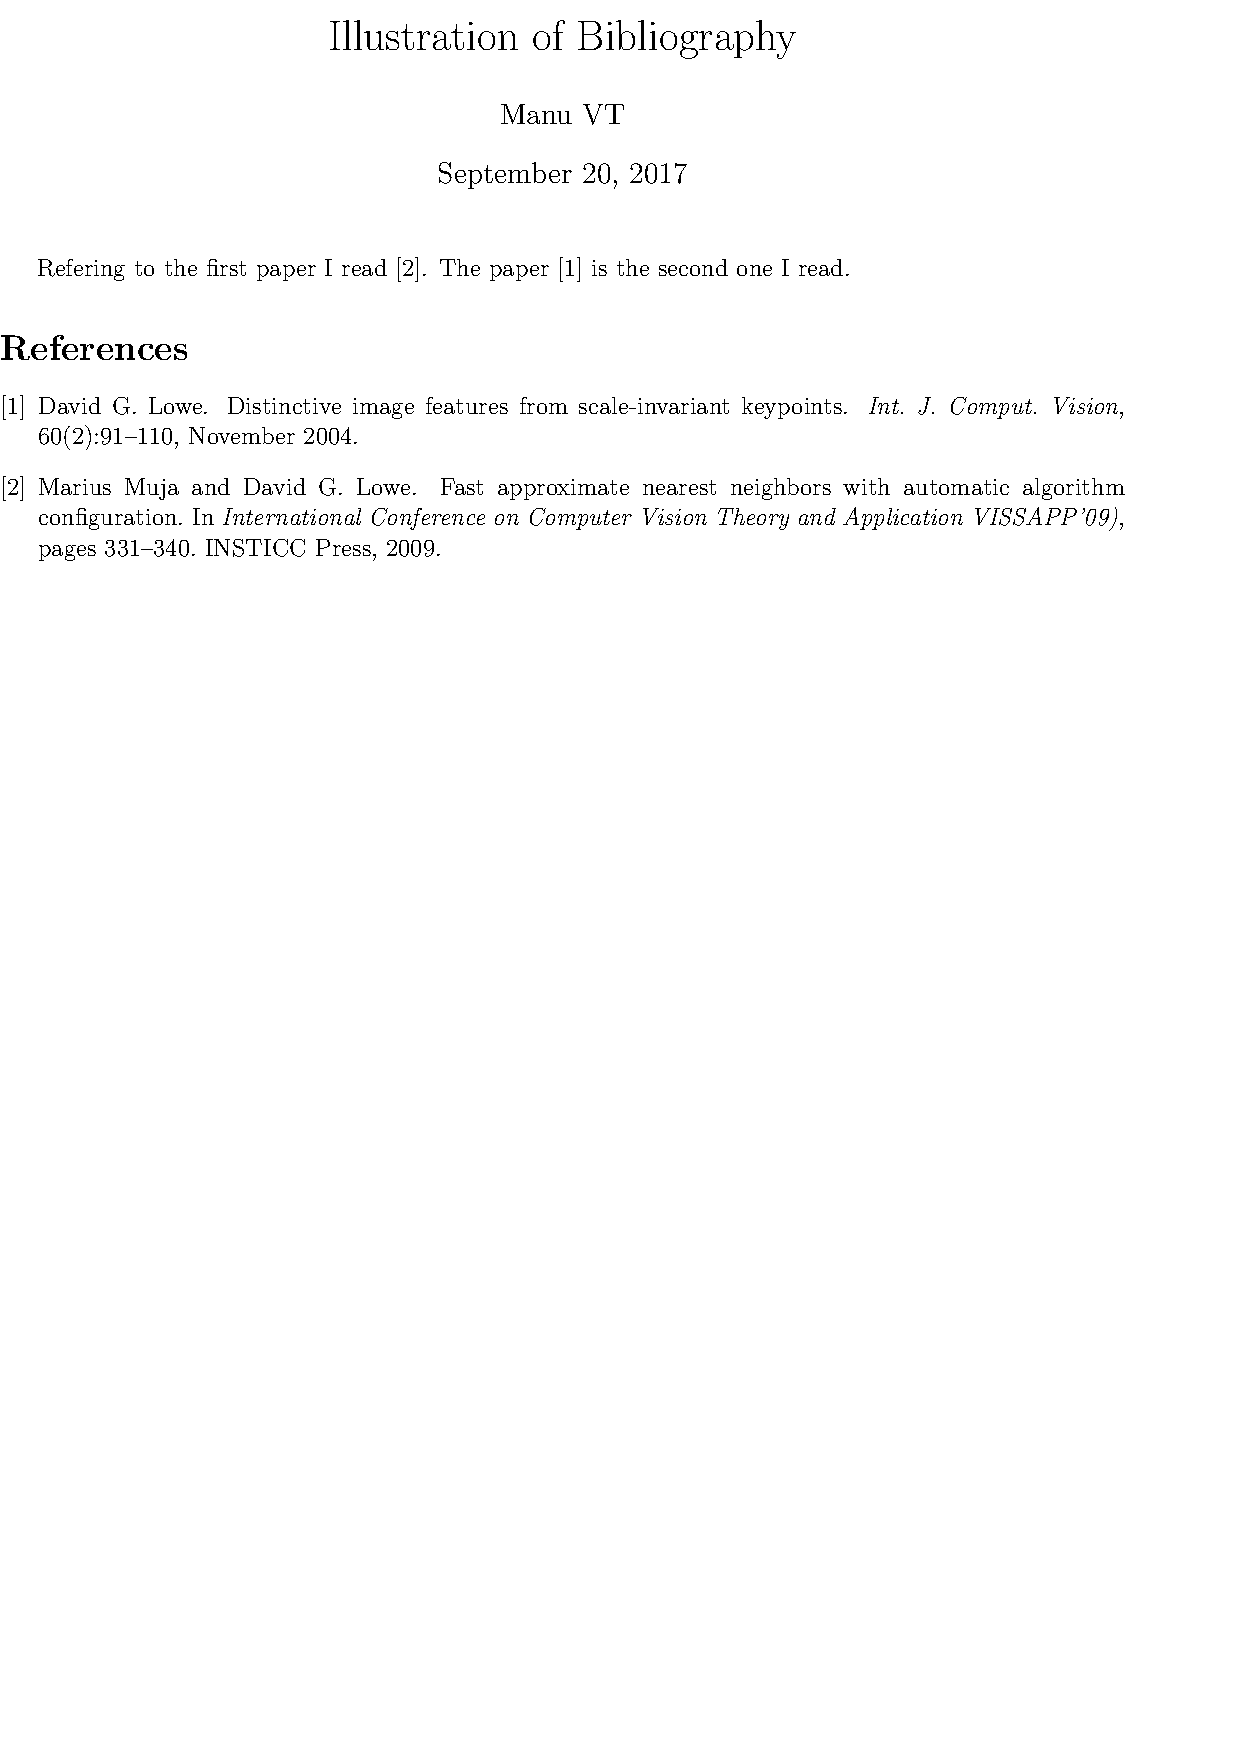
\includegraphics[scale=0.6]{biblio_example}
\end{frame}
%%%%%%%%%%%%%%%%%%%%%%%%%%%%%%%%%%%%%%%%%%%%%%%%%%%%%%%%%%%%%%%%%%%%%%%%%%%%%%%%%%%%%%%%%%%%%%%%%%%%%%%%%%%%%%%%%%%%%%%%%%%%%
%%%%%%%%%%%%%%%%%%%%%%%%%%%%%%%%%%%%%%%%%%%%%%%%%%%%%%%%%%%%%%%%%%%%%%%%%%%%%%%%%%%%%%%%%%%%%%%%%%%%%%%%%%%%%%%%%%%%%%%%%%%%%
\begin{frame}[shrink=20,fragile]			
\begin{verbatim}
\title{Illustration of Bibliography}
\author{Manu VT}

\begin{document}

\maketitle

Refering to the first paper I read \cite{muja_flann_2009}.
The paper \cite{Lowe:2004:DIF:993451.996342} is the second 
one I read.



%\bibliographystyle{elsarticle-harv}
\bibliographystyle{plain}
\bibliography{bib}
\end{document}
\end{verbatim}
\end{frame}
%%%%%%%%%%%%%%%%%%%%%%%%%%%%%%%%%%%%%%%%%%%%%%%%%%%%%%%%%%%%%%%%%%%%%%%%%%%%%%%%%%%%%%%%%%%%%%%%%%%%%%%%%%%%%%%%%%%%%%%%%%%%%\\
%%%%%%%%%%%%%%%%%%%%%%%%%%%%%%%%%%%%%%%%%%%%%%%%%%%%%%%%%%%%%%%%%%%%%%%%%%%%%%%%%%%%%%%%%%%%%%%%%%%%%%%%%%%%%%%%%%%%%%%%%%%%%
\begin{frame}[fragile,shrink=20]
\section{How to Create a Bibiliography File?         }
\frametitle{Bibiliography File}
\begin{itemize}\justifying
	\item .bib format
	\item 
	\begin{verbatim}
	@article{Lowe:2004:DIF:993451.996342,
	author = {Lowe, David G.},
	title = {Distinctive Image Features from Scale-Invariant Keypoints},
	journal = {Int. J. Comput. Vision},
	issue_date = {November 2004},
	volume = {60},
	number = {2},
	month = nov,
	issn = {0920-5691},
	pages = {91--110},
	year = {2004},
	doi={10.1023/B:VISI.0000029664.99615.94}
	} 
	
	@inproceedings{muja_flann_2009,
	author    = {Marius Muja and David G. Lowe},
	title     = {Fast Approximate Nearest Neighbors with Automatic Algorithm Configuration},
	booktitle = {International Conference on Computer Vision Theory and Application 
	VISSAPP'09)},
	publisher = {INSTICC Press},
	year      = {2009},
	pages     = {331-340}
	}
	
	\end{verbatim}
\end{itemize}
\end{frame}
%%%%%%%%%%%%%%%%%%%%%%%%%%%%%%%%%%%%%%%%%%%%%%%%%%%%%%%%%%%%%%%%%%%%%%%%%%%%%%%%%%%%%%%%%%%%%%%%%%%%%%%%%%%%%%%%%%%%%%%%%%%%%\\

%%%%%%%%%%%%%%%%%%%%%%%%%%%%%%%%%%%%%%%%%%%%%%%%%%%%%%%%%%%%%%%%%%%%%%%%%%%%%%%%%%%%%%%%%%%%%%%%%%%%%%%%%%%%%%%%%%%%%%%%%%%%%
\begin{frame}
\section{Exporting Citations from Scholarly Research Databases}
\frametitle{Exporting Citations from Scholarly Research Databases}

\includegraphics[scale=0.35]{Exporting_Citation1}

\end{frame}
%%%%%%%%%%%%%%%%%%%%%%%%%%%%%%%%%%%%%%%%%%%%%%%%%%%%%%%%%%%%%%%%%%%%%%%%%%%%%%%%%%%%%%%%%%%%%%%%%%%%%%%%%%%%%%%%%%%%%%%%%%%%%
\begin{frame}
\frametitle{Exporting Citations from Scholarly Research Databases}
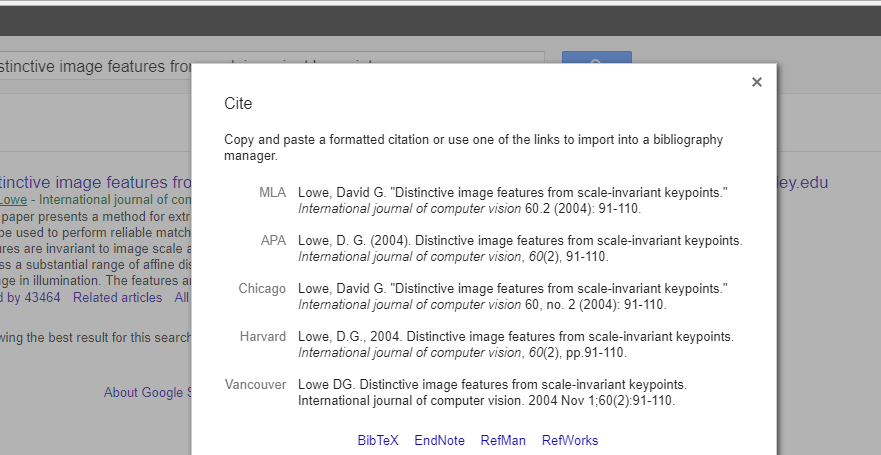
\includegraphics[scale=0.35]{Exporting_Citation2}
\end{frame}
%%%%%%%%%%%%%%%%%%%%%%%%%%%%%%%%%%%%%%%%%%%%%%%%%%%%%%%%%%%%%%%%%%%%%%%%%%%%%%%%%%%%%%%%%%%%%%%%%%%%%%%%%%%%%%%%%%%%%%%%%%%%%
\begin{frame}
\frametitle{Exporting Citations from Scholarly Research Databases}

\includegraphics[scale=0.35]{Exporting_Citation3}
\end{frame}
%%%%%%%%%%%%%%%%%%%%%%%%%%%%%%%%%%%%%%%%%%%%%%%%%%%%%%%%%%%%%%%%%%%%%%%%%%%%%%%%%%%%%%%%%%%%%%%%%%%%%%%%%%%%%%%%%%%%%%%%%%%%%
\begin{frame}[fragile,shrink=20]
\section{}
\frametitle{More on Bibliographic Files}
\begin{itemize}
	\item .bbl file
	\item Editing .bbl file and direct inclusion in .tex file.
\end{itemize}
\begin{verbatim}
\begin{thebibliography}{1}

\bibitem{Lowe:2004:DIF:993451.996342}
David~G. Lowe.
\newblock Distinctive image features from scale-invariant keypoints.
\newblock {\em Int. J. Comput. Vision}, 60(2):91--110, November 2004.

\bibitem{muja_flann_2009}
Marius Muja and David~G. Lowe.
\newblock Fast approximate nearest neighbors with automatic algorithm
configuration.
\newblock In {\em International Conference on Computer Vision Theory and
Application VISSAPP'09)}, pages 331--340. INSTICC Press, 2009.

\end{thebibliography}

\end{verbatim}
\end{frame}
%%%%%%%%%%%%%%%%%%%%%%%%%%%%%%%%%%%%%%%%%%%%%%%%%%%%%%%%%%%%%%%%%%%%%%%%%%%%%%%%%%%%%%%%%%%%%%%%%%%%%%%%%%%%%%%%%%%%%%%%%%%%%
\begin{frame}[fragile,shrink=20]
\section{}
\frametitle{More on Bibliographic Files}
\begin{itemize}
	\item .aux file
	\item Recreating .aux file. 
\end{itemize}
\begin{verbatim}
\relax 
\citation{muja_flann_2009}
\citation{Lowe:2004:DIF:993451.996342}
\bibstyle{plain}
\bibdata{bib}
\bibcite{Lowe:2004:DIF:993451.996342}{1}
\bibcite{muja_flann_2009}{2}
\end{verbatim}
\end{frame}
%%%%%%%%%%%%%%%%%%%%%%%%%%%%%%%%%%%%%%%%%%%%%%%%%%%%%%%%%%%%%%%%%%%%%%%%%%%%%%%%%%%%%%%%%%%%%%%%%%%%%%%%%%%%%%%%%%%%%%%%%%%%
 \begin{frame}
 \frametitle{Tools for Bibliography}
\begin{itemize}\justifying
	\item  Zotero\\
	
\includegraphics[scale=0.25]{zotero_logo}
	\item Mendeley\\
		
\includegraphics[scale=0.25]{mendeley}
\end{itemize}
\end{frame}
%%%%%%%%%%%%%%%%%%%%%%%%%%%%%%%%%%%%%%%%%%%%%%%%%%%%%%%%%%%%%%%%%%%%%%%%%%%%%%%%%%%%%%%%%%%%%%%%%%%%%%%%%%%%%%%%%%%%%%%%%%%%%
%%%%%%%%%%%%%%%%%%%%%%%%%%%%%%%%%%%%%%%%%%%%%%%%%%%%%%%%%%%%%%%%%%%%%%%%%%%%%%%%%%%%%%%%%%%%%%%%%%%%%%%%%%%%%%%%%%%%%%%%%%%%%%
\begin{frame}
 \begin{center}
\begin{block}{}
\hspace*{2in}\textbf{\LARGE \textcolor{idrbt_dark_blue}{T}\pause
			    \textcolor{idrbt_blue}{h}\pause
			    \textcolor{idrbt_dark_blue}{a}\pause
			    \textcolor{idrbt_blue}{n}\pause
			    \textcolor{idrbt_dark_blue}{k}\pause
			    \textcolor{idrbt_dark_blue}{Y}\pause
			    \textcolor{idrbt_blue}{o}\pause
			    \textcolor{idrbt_dark_blue}{u} }
\end{block}\end{center}
\end{frame}
\end{document}
%%%%%%%%%%%%%%%%%%%%%%%%%%%%%%%%%%%%%%%%%%%%%%%%%%%%%%%%%%%%%%%%%%%%%%%%%%%%%%%%%%%%%%%%%%%%%%%%%%%%%%%%%%%%%%%%%%%%%%%%%%%%%